\section{Autoregressive model in case of multiple damage}\label{methodology_twostage}

The proposed two-stage procedure is based on signal filtering. Here we use both autoregressive modeling and optimal frequency band selection. Sometimes, the raw vibration signal contains a strong deterministic contamination which is highly amplitude modulated. In such case of time varying signal-to-noise ratio the signal of interest is invisible in both time series and envelope spectrum. Then, signal filtering based on measures of dispersion (e.g. the spectral kurtosis) may indicate a wrong frequency band as informative. We propose to filter out the deterministic signal using autoregressive filtering. The next step is based on linear filtering using frequency characteristics of the filter obtained by measures of impulsiveness. We compare filters driven by the spectral kurtosis~\cite{Combet2009652} and one of informative frequency band selectors presented in~\cite{Obuchowski2013441,Obuchowski2013,Obuchowski2014138}.
As it was mentioned, we use the autoregressive model to filter out highly amplitude modulated mesh harmonics. The AR model of order $p$ is defined as follows:
\begin{equation}
\sum_{i=0}^p\phi(i)X(t-i)=\epsilon(t),
\end{equation}
where $\phi(0)=0$ and $\epsilon(t)$ stands for noise.\\
It is known, that the AR time series model is able to model noisy sinusoidal pattern if its characteristic polynomial has complex roots. In the case of a large number of harmonics a high-order AR model is expected with at least two complex roots corresponding to one mesh harmonic. As the optimal order indicator we use the highest Kolmogorov-Smirnov criterion, i.e. $\mathrm{AR}(p)$ is said to be optimal if the Kolmogorov-Smirnov (KS) test statistic of residuals is the highest~\cite{Zhan20071953}. According to the fact that the residual signal in case of local damage should be impulsive, it is expected that the distance between empirical distribution and Gaussian one is high – the higher KS statistic, the more impulsive signal. Recall the KS statistic for signal $X(t)$ is defined as follows~\cite{Justel1997251}:
\begin{equation}
KS=\sup{x}\left|\hat{F}(x)-F(x)\right|,
\end{equation}
where $\hat{F}(x)$ is the empirical cumulative distribution function for given signal while $F(x)$ is the cumulative distribution function of Gaussian distribution with parameters estimated form the signal.\\
Moreover, the results of AR filtering are also checked by comparing time-frequency maps of the residual signal with the raw signal. Parameters of the AR model are obtained by using Yule-Walker~\cite{Brockwell1991}.
Fig.~\ref{twostage_fig01}
\begin{figure}[ht]
\begin{center}
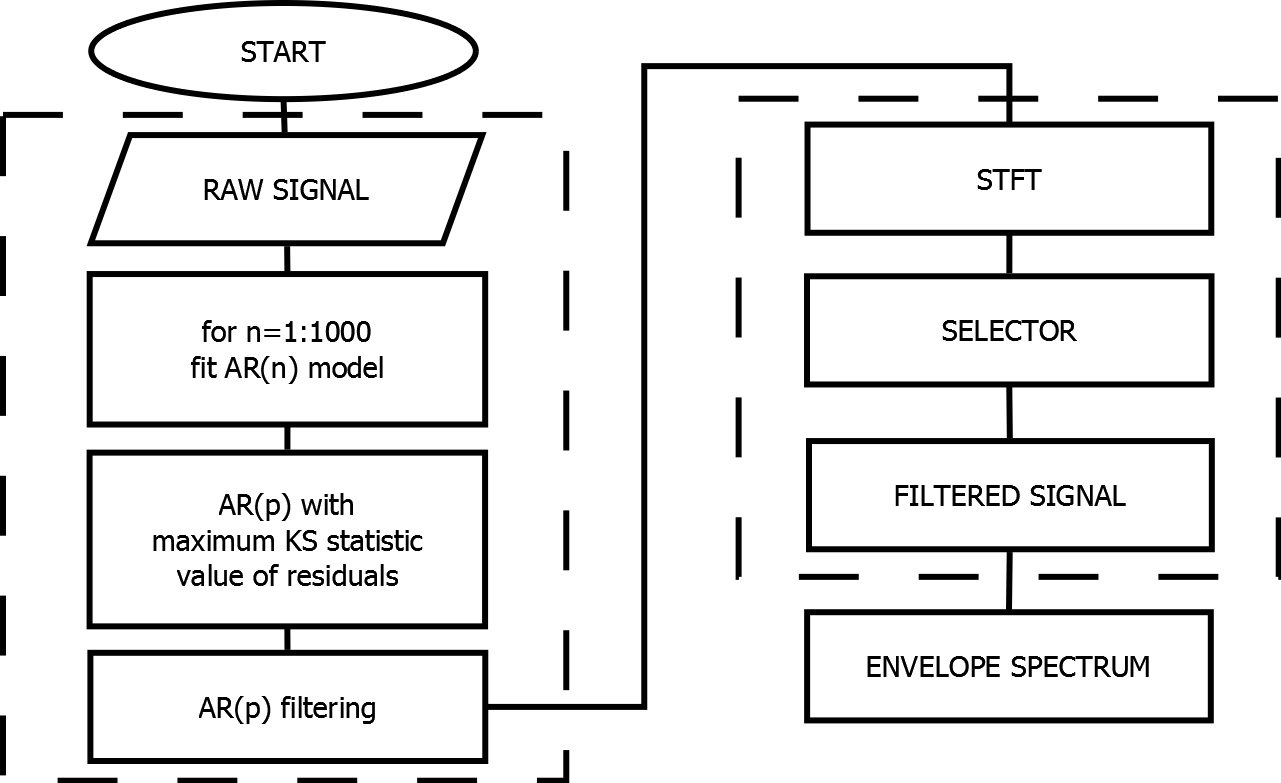
\includegraphics[width=0.7\textwidth]{methodology/twostage/twostage_diagram}
\caption{Block diagram of the two-stage procedure}\label{twostage_fig01}
\end{center}
\end{figure}
Once mesh harmonics are suppressed during the previous step of the procedure, the residual signal might be still noisy, e.g. when the SOI is relatively narrowband. We propose to select the informative frequency band using the average horizontal distance on quantile-quantile plot (QQplot)~\cite{Obuchowski2013441,Obuchowski2013,Obuchowski2014138}. Namely, we quantify the average distance between markers and reference line on the QQplot. The QQplot we use here is a graphical goodness-of-fit tool which compares quantiles of empirical distribution of the sample with the Gaussian distribution. The reference line connects first and third quartiles of both distributions. We compare it to the well-known spectral kurtosis. Both of them are based on analysis of narrowband slices of a time-frequency map. In this paper we design the filter using not only the characteristic given by a selector but we also enhance the characteristic by using individual thresholds of selector's value for a given frequency bin. Namely, we put 0 in the frequency characteristic of the filter if the value of the selector is lower than the threshold for a given frequency bin. The thresholds are obtained using the Monte Carlo method and inverse pre-whitening~\cite{Obuchowski2013}.\\
After designing the filter, we filter out the residual signal by computing Fourier transform of the signal, multiplying it by frequency response of the selector-based filter and, finally, using the inverse Fourier transform to return to the time domain. This method is an extension of the method presented in~\cite{Combet2009652}, where the filter is constructed using the spectral kurtosis.\\
A block diagram of our two-stage procedure is presented in Fig.~\ref{twostage_fig01}.
\FloatBarrier